\section{Technical Implementation}

% Do these need references?
Discovery Service is implemented with Python programming language and Flask Web framework. They were chosen because all of the components in Cloudify are also written in Python and Flask is used primarily for providing REST APIs. Even though Discovery Service does not provide any REST APIs, Flask is used for configuration management and source code organisation. Naturally, if need arises in the future to expand Discovery Service with a REST API, the development work is streamlined because of the framework.

In addition to Python program, Discovery Service relies on Redis \cite{Redis} as an in-memory key-value storage. Redis is a completely separate process in addition to Discovery Service. The preferred way of deploying Redis is in a docker container as it doesn't require installation or configuration save for exposing a correct port in the container and specifying Redis' address to Discovery Service. Redis could also be installed in the host system or even a remote system, though latter option has no practical purpose due to network latency as Redis achieves its high performance by storing values in the memory instead of disk.

\begin{figure}[ht!]
\centering
  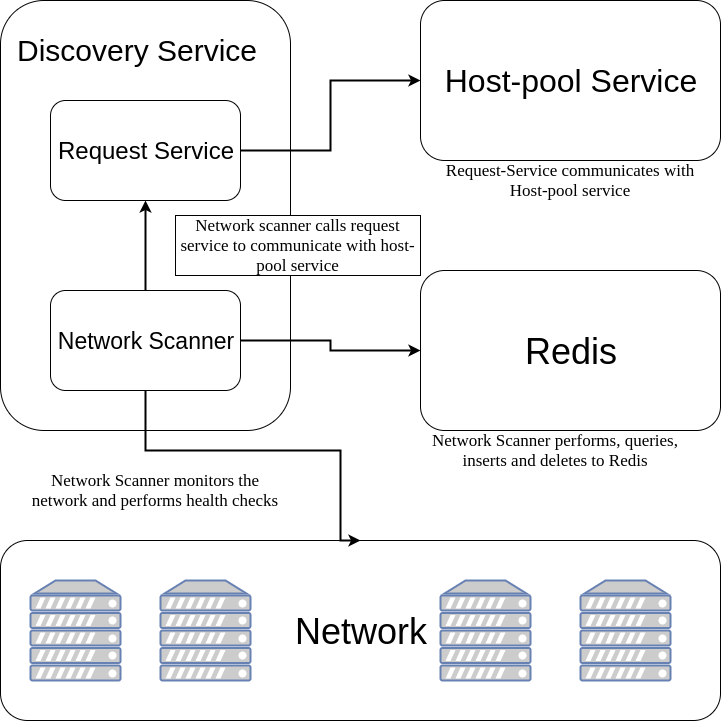
\includegraphics[width=12cm,height=12cm, keepaspectratio]{Discovery-service-communication.png}
  \caption{The communication relationships between Discovery Service and other components}
  \label{fig:communications}
\end{figure}

On the source code level, Discovery Service consists of two major components: The network scanner and request service. The network scanner is given a subnet as a parameter and it constantly sniffs the network detecting joining and already present devices and keeping track of them. Its other task is to periodically send health checks to known devices and if a health check fails enough times, it removes the given device from the logical host pool. Request service is responsible for sending HTTP requests to the Cloudify Host-pool service. It is called by the request service and it runs asynchronously. In addition to HTTP requests, it performs checks to ensure that the state of Discovery service's and Host-pool service's databases correlate.

The communication relationships between different components in the system are depicted in figure \ref{fig:communications}. The source code for Discovery Service as well as the documentation can be found at \url{https://bitbucket.org/Fleuri/discoveryserviceforcloudify/src/master/}

\subsection{Network Scanner}

The Network Scanner has two main functions, sniffer and pinger, and they run concurrently on two threads. Sniffer listens to ARP packets in the network and upon receiving one, stores the details of the sender device. Pinger function periodically sends ARP pings to previously discovered device and keeps track of their successes, eventually removing unresponsive devices from the logical host pool. In addition to two main functions there's a startup function that initialises both local Redis storage and the Host-pool service's database. It pings all of the IP addresses in the given IP range and stores the found device details to databases.

\subsubsection{Sniffer}

\subsubsection{Pinger}

\subsection{Request Service}

